% !TEX root = BA-Bauer

\subsection{STMicroelectronics STM32F446ZE}
\label{sec:STM}
Aufgrund der aktuellen Corona-Pandemie und einer damit einhergehenden Siliziumchip-Knappheit wird für die Entwicklung ein anderer Mikrocontroller als in der Praxisarbeit verwendet. Die Eckdaten beider Mikrocontroller sind sich trotzdem sehr ähnlich. Abbildung \ref{fig:MCU_pinout} zeigt die Pinbelegung des Chips. Insgesamt stehen 114 interruptfähige Ein- und Ausgangsports, von denen 112 5\,V Tolerant sind und bis zu 20 Schnittstellen zur Verfügung. Der interne 512\,Kbytes große Flash-Speicher und 128\,Kbyte SRAM bieten genügend Kapazität für einen großen Programmcode, sowie genügend Platz für Heap und Stack. Der STM32F446ZE arbeitet mit einer maximalen Taktfrequenz von 180MHz und basiert auf einem \textit{Arm\textsuperscript{®} 32-bit Cortex\textsuperscript{®}-M4} Prozessor \cite[S. 1]{STM32F446ZE_Datasheet}.
\begin{figure}[!htb]
	\begin{center}
		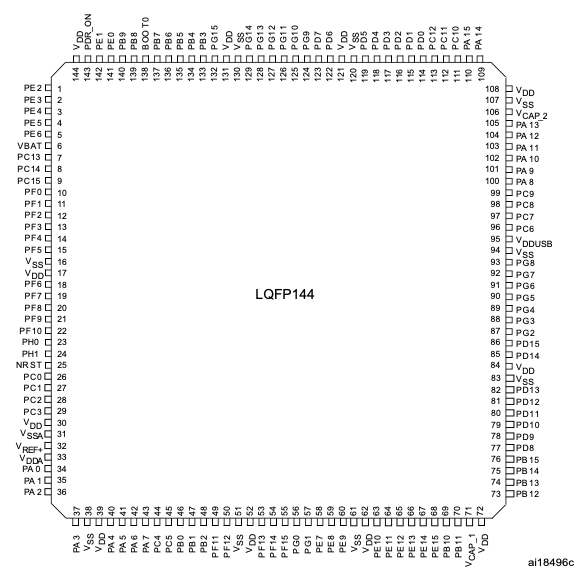
\includegraphics[scale = 0.4]{STM32F446ZE_pinout}
		\caption{STMicroelectronics STM32F446ZE Mikrocontroller Pinout \cite[S. 41]{STM32F446ZE_Datasheet}}
		\label{fig:MCU_pinout}
	\end{center}
\end{figure}\\
\newline
\hspace{-5mm}\textbf{Spannungsversorgung}\\
Die Spannungsvesorgung des MCUs ist besonders kritisch, da eine einbrechende Spannung zu Fehlern bei der Ausführung des Programmcodes oder sogar zu einem kurzzeitigen Ausfall und Neustart des MCUs führen kann. Bei steigenden Schaltfrequenzen des MCUs wirken die Leiterbahnen auf der Platine induktiv, wodurch möglicherweise nicht schnell genug genügend Strom geliefert werden kann, was zu einem Einbruch der Spannung führen kann. Um dem entgegenzuwirken werden sogenannte Stützkondensatoren möglichst nah an den Versorgungsspannungs-Pins ($V\textsubscript{DD}$ und $V\textsubscript{SS}$) des MCUs plaziert. Benötigt der MCU kurzzeitig einen großen Strom, so entlädt sich der Kondensator. Durch die kurze Distanz zum MCU muss der Strom über eine kürzere Strecke der Leiterbahn fließen, was eine niedrige Induktivität zur Folge hat. Im Datenblatt \cite{F446RM} des MCUs kann die Dimensionierung der Stützondensatoren entnommen werden. Insgesamt werden elf Pin-Paare, bestehen aus VDD (3,3\,V) und VSS (0\,V) mit 0,1\,$\mu$F Kondensatoren parallel verbunden.\\
\newline
\textbf{Taktgeber (Clock)}\\
Der MCU verfügt über einen internen hochgeschwindigkeits-Oszillator \textit{High-Speed-Internal-Clock} (HSI) und einen niedergeschwindigkeits-Oszillator \textit{Low-Speed-Internal-Clock} (LSI). Die HSI schwing mit einer Frequenz von 16\,MHz und ist werksseitig auf eine Abweichung der Schwingfrequenz von einem Prozent kalibriert. Um die maximale Taktfrequenz des Prozessors zu erreichen wird eine interne Phasenregelschleife (PLL) eingesetzt. Durch die PLL kann ein Vielfaches der Oszilatorfrequenz erzeugt werden, wobei die Stabilität der Schwingung nicht eingeschränkt wird \cite[S. 270]{Ehrhardt1992}. Eine weitere Möglichkeit die Taktfrequenz zu genrieren, ist die Verwendung eines externen Oszilators (HSE). Der in dieser Arbeit verwendete externe Quartz schwingt mit einer Frequenz von 25\,MHz und hat dabei eine Genaigkeit von 30\,ppm. Das entpricht einer maximalen Abweichung von ca. \(30*10^{-6}\)\,\%, also einer deutlich geringeren Abweichung im Vergleich zum internen Oszilator. Da für die Aufnahme und Wiedergabe der DMX-Daten möglichst genaue Zeitabstände benötigt werden, wird der externe Quartz verwendet.
\begin{figure}[!h]
	\begin{center}
			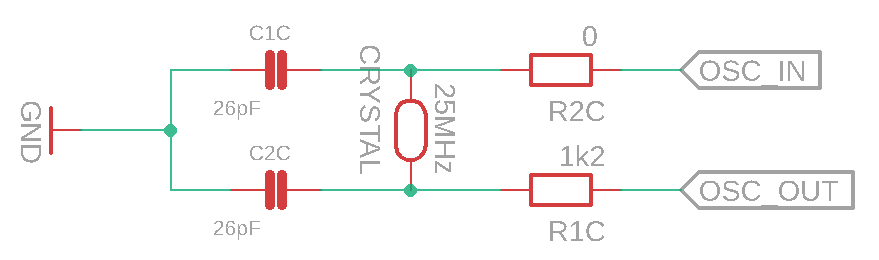
\includegraphics[scale=1]{Schaltung-Quartz}
			\caption{Beschaltung Quartz}
			\label{fig:Quartz}
	\end{center}
\end{figure}\\
Abbildung \ref{fig:Quartz} zeigt die Beschaltung des externen Quartzes. Er wird parallel zu dem Eingang $OSC\_IN$ und dem Ausgang $OSC\_OUT$ des MCUs geschaltet. Zwischen dem Ein- und Ausgang des MCUs befindet sich ein integriertes \textit{Nicht-Gatter} (Inverter) \cite[S. 11]{OscillatorAN}, welcher bei einem Schaltvorgang hohe Ströme ausgeben kann. Damit kein Schaden am Quartz und MCU entsteht, wird der maximal fließende Strom durch den Widerstand \textit{R1C} am $OSC\_OUT$-Pin begrenzt. Aus Symmetriegründen befindet sich ein 0\,$\Omega$-Widerstand am $OSC\_IN$-Pin, der dafür sorgt, dass auf beiden Seiten des Quartzes die gleichen Übergangskapazitäten der Lötstellen vorhanden sind. Der Quartz wird mithilfe von zwei Lastkapazitäten mit dem 0\,V Potential verbunden. Der Wert der Kapazitäten \textit{$C_{L1}$} und \textit{$C_{L2}$} lässt sich mit folgender Formel berechnen.
\begin{equation}
		C_L = \frac{C_{L1} * C_{L2}} {C_{L1} + C_{L2}} + C_s \cite[S. 12]{OscillatorAN}
\end{equation}
\textit{$C_L$} wird vom Hersteller des Quartzes vorgegeben und beträgt in diesem Fall 18\,pF. \textit{$C_S$} ist die Kapazität der Lötstellen und Leiterbahnen zwischen dem Quartz und dem MCU, welche mit 5\,pF angenommen wird. Um möglichst wenig verschiedene Bauteile verwenden zu müssen, erhalten in der Regel die Kapazitäten $C_{L1}$ und $C_{L2}$ die gleiche Wertigkeit, wodurch die Formel wie folgt vereinfacht werden kann.
\begin{equation}
	C_{L1} =  C_{L2} = 2(C_L - C_S)
\end{equation}
Laut der Formel müssen $C_{L1}$ und $C_{L2}$ eine Kapazität von 26\,pF aufweisen. Da Kondensatoren mit dieser Kapazität nur schwer erhältlich sind wird eine marktüblichere Kapazität von 27\,pF verwendet.\\
\newline
\textbf{Serial Wire Debug-Schnittstelle (SWD)}\\
Im Auslieferungszustand des MCUs befindet sich keine Software auf diesem. Mit einem Entwicklungsboard, wie es in der Praxisarbeit verwendet wurde, kann eine Software einfach über eine USB-Schnittstelle auf den MCU übertragen werden, da auf dem Entwicklungsboard ein sogenannter $programmer$ verbaut ist. Das in der Praxisarbeit verwendete Entwicklungsboard bietet die Möglichkeit einen Teil der Platine abzutrennen und als eigenständigen $programmer$ zu verwenden mit dem die Software mithilfe der \textit{Serial Wire Debug}-Schnittstelle (SWD-Schnittstelle) auf den MCU übertragen werden kann. Die SWD-Schnittstelle ermöglicht das Übertragen der Software und das Debuggen\footnote{Analyse und Fehlerbehebung von Programmcode} des Codes während der Laufzeit. Für die Datenübertragung zwischen MCU und PC werden nur zwei Verbindungen (SWD und SWCK) benötigt. Über die Leitung SWD werden die Daten gesendet wohingegen die Leitung SWCK den Takt des Datenstroms angibt. Soll ein neues Programm auf den MCU übertragen werden, so muss er zunächst in einen speziellen Modus versetzt werden, um den Programmspeicher beschreiben zu können. Dazu muss der MCU neugestartet werden und beim Start des MCU am $BOOT0$-Pin ein High-Pegel anliegen. Sobald die Übertragung beendet ist, muss der MCU ein weiteres Mal neugestartet werden um den Programmcode auszuführen, jedoch muss beim Start nun ein Low-Pegel am $BOOT0$-Pin anliegen. Das Anlegen der entsprechenden Pegel am $BOOT0$-Pin sowie der Neustart kann per Hand durchgeführt werden, jedoch kann diese Aufgabe auch von dem $programmer$ übernommen werden. Dafür müssen zwei weitere Verbinungen für den $BOOT0$-Pin und $NRST$-Pin vorhanden sein. Zuletzt ist außerdem eine Verbindung des 0\,V-Potentials notwendig da es sich bei allen Signalen um spannungsbezogene Signale handelt. Optional kann der MCU mit einer weiteren Verbindung vom $programmer$ mit 3,3\,V Spannung versorgt werden.\\
\newline
\textbf{NRST- und BOOT0-Pin}\\
Unter den 144 Pins des MCUs befinden sich unter anderem, wie bereits im vorigen Abschnitt erwähnt, der $NRST$- und $BOOT0$-Pin. Beide Pins sind mit externen Tastern beschaltet um Fehler bei den Verbindungen zwischen MCU und $programmer$ zu kompensieren. Außerdem kann das Programm mit dem Betätigen eines Tasters neugestartet werden, was bei der programmierung von Vorteil ist. Für den verkaufsfertigen Zustand des Gerätes werden die Taster allerdings nicht mehr benötigt und können einfach weggelassen werden. 